%\documentclass[10pt, twocolumn]{article}
\documentclass[twocolumn,showpacs,preprintnumbers,amsmath,amssymb,prd]{revtex4}
%\documentclass[11 pt,preprint,preprintnumbers,amsmath,amssymb, prd]{revtex4}

% Preamble adapted from Surjeet Rajendran

\usepackage{latexsym}
\usepackage{amssymb}
\usepackage{epsfig,amsmath,graphics}
\usepackage{epstopdf}
\usepackage{verbatim}
\usepackage{wasysym}
\usepackage{hyperref}
\usepackage{feynmp-auto} % feynman diagrams
%\usepackage{subfig}
\usepackage[utf8]{inputenc}
\usepackage{xpatch}
\usepackage{xcolor}
\hypersetup{
    colorlinks,
    linkcolor={red!80!black},
    citecolor={green!60!black},
    urlcolor={blue!60!black}
}
\usepackage{appendix}

\newcommand{\OO}{\mathcal{O}}
\newcommand{\LL}{\mathcal{L}}
\newcommand{\HH}{\mathcal{H}}

\newcommand{\GeV}{\text{GeV}}
\newcommand{\MeV}{\text{MeV}}
\newcommand{\keV}{\text{keV}}
\newcommand{\rad}{\text{rad}}
\newcommand{\cm}{\text{cm}}
\newcommand{\angstrom}{\buildrel _{\circ} \over {\mathrm{A}}}
\newcommand{\pslash}{p\hspace{-0.070in}/\,}
\newcommand{\Mpl}{M_{\text{pl}}}
\newcommand{\ket}[1]{\ensuremath{\left|#1\right>}}
\newcommand{\bra}[1]{\ensuremath{\left<#1\right|}}
\newcommand{\braket}[2]{\ensuremath{\left<#1|#2\right>}}
%Large Parentheses
\def\r{\right)}
\def\l{\left(}

\begin{document}

\title{White Dwarfs as Dark Matter Detectors}


\author{Ryan Janish}
\affiliation{Berkeley Center for Theoretical Physics, Department of Physics,
University of California, Berkeley, CA 94720, USA}

\author{Vijay Narayan}
\affiliation{Berkeley Center for Theoretical Physics, Department of Physics,
University of California, Berkeley, CA 94720, USA}

\author{Paul Riggins}
\affiliation{Berkeley Center for Theoretical Physics, Department of Physics,
University of California, Berkeley, CA 94720, USA}

\begin{abstract}

White dwarfs can serve as detectors for ultra-heavy dark matter states which interact to trigger type Ia supernovae. This was originally proposed in \cite{Graham:2015apa} and used to  place bounds on primordial black holes. In this paper we extend the capability of white dwarf detectors to candidates with non-gravitational couplings, focusing on dark matter transits and collisions within the white dwarf. In particular, we provide a detailed analysis of the explosiveness for any heating mechanism in the white dwarf which releases high-energy standard model particles. We apply this mechanism to constrain Q-ball dark matter \textcolor{blue}{and model of dark nuclei} in regions of parameter space fundamentally inaccessible to terrestrial-based experiments. 

\end{abstract}
\maketitle


\section{Introduction}
\label{sec:Introduction}

The detection of ultra-heavy dark matter (DM) is an open problem which will ultimately require a confluence of astrophysical probes. For instance, DM masses above $\sim 10^{22} ~\GeV$ will register fewer than 1 event per year in a typical terrestrial detector of size $\sim (100 ~\text{m})^2$. Furthermore, the lack of conclusive signatures on a variety of experimental fronts has led many to seriously consider DM candidates far above the weak scale and their potential signatures \textcolor{blue}{cite people}. One possibility proposed by \cite{Graham:2015apa} is that ultra-heavy DM can trigger supernovae in sub-Chandrasekhar white dwarf (WD) stars by inducing runaway fusion.  In this regard, white dwarfs can serve as detectors for ultra-heavy DM states.

White dwarfs are particularly suited to this task, as they are more susceptible to runaway fusion than are main-sequence stars. Runaway fusion requires that two criteria be met: a region within the star must be hot enough to support exothermic fusion reactions, and the rate at which energy is released by these reactions must dominate any cooling mechanisms that drain energy from the fusing region.  The stellar medium of a WD has fewer cooling mechanisms available than does a non-degenerate star - WD cooling relies on thermal diffusion whereas main-sequence stars can also cool via thermal expansion.  This is suppressed in a WD since its pressure is determined by electron degeneracy and is thus independent of temperature. The remaining primary cooling mechanism, diffusion, becomes less important over longer length scales and can be overcome by sufficiently heating a large enough region of the WD. 

The necessary trigger for runaway fusion was initially computed in \cite{Woosley} and subsequently implemented in \cite{Graham:2015apa} to constrain primordial black holes, which can ignite WD stars via gravitational dynamical friction.  In addition, the authors of \cite{Graham:2015apa} identify several other heating mechanisms involving DM which may be constrained in a similar manner.  \textcolor{blue}{Some of these have been explored in follow-up works...citations, citations.}  In this work, we extend their analysis to DM candidates with generic non-gravitational couplings, focusing on DM transits through the WD and DM-DM collisions within the WD which release energy in the form of standard model (SM) particles. More generally, we provide a detailed analysis of the explosive power and resulting constraints on any DM with interactions of this sort. 

Concrete examples of DM candidates with interactions of this type include baryonic Q-balls found in supersymmetric extensions of the SM and \textcolor{blue}{dark nuclei with high-order couplings to the SM.} We are able to constrain these models in regions of parameter space fundamentally inaccessible to terrestrial experiments. However, it is important to note that any such DM constraints are by nature complimentary to terrestrial ones - it is more massive DM that is likely to trigger supernovae, and also more massive DM that have sufficiently low flux on Earth. What allows the WD to be effective in this regime is its enhanced surface area $\sim (4000 ~\text{km})^2$ and exceptionally long lifetime $\sim \text{Gyr}$. In this sense, the WD is a large ``space-time volume" detector. \textcolor{blue}{We also have a ``flux is too low" limit...should we include here?}

\textcolor{blue}{Other ignition sources exist (i.e., detector backgrounds). How does this limit our constraints? Discuss the specific tests we apply (WD lifetime, SN rate) to derive our constraints.} \textcolor{red}{Possible long term addition: improve constraints by using non-type IA sn rate instead of total rate. Should talk with SN people first.}

We begin in Section \ref{sec:review} by reviewing the explosion mechanism in a WD. In Section \ref{sec:DMexplode}, we parametrize the properties of DM necessary to trigger explosions through non-gravitational interactions in the case of a DM transit or collision in the star. The precise explosive power will be determined by a heating length, which is computed in \ref{sec:heatinglength} for different possible interactions. Following this general discussion, we apply the WD detector to constrain Q-balls in Section \ref{sec:Qballs} and conclude in Section \ref{sec:discussion}. 

\section{White Dwarf Runaway Fusion}
\label{sec:review}
In a WD, the \emph{fusion temperature} $T_f$ is a constant set by the energy required for ions to overcome their mutual Coulomb barriers $T_f \sim \MeV$. WD cooling is set by the thermal diffusivity of photons and degenerate electrons. The two species dominate the cooling at different stellar densities, as determined precisely in \cite{Woosley}. Note that for a heated region of size $R$, this cooling rate scales as $R^{-2}$ while the fusion rate scales as $R^{-3}$. Thus there is a critical \emph{trigger size} $\lambda_T$ below which diffusive cooling dominates the thermal evolution of a temperature peak, and above which the liberated fusion energy dominates \cite{Woosley}. Therefore, a region with temperature greater than $T_f$ and size greater than $\lambda_T$ in a given WD will launch a runaway fusion chain-reaction and result in a type Ia supernova. The numerical value of $\lambda_T$ is highly sensitive to the WD density and has been analytically scaled for varying WD masses in \cite{Graham:2015apa}. As in \cite{Graham:2015apa}, we restrict our attention to carbon-oxygen WDs in the upper mass range $0.7 - 1.4 ~M_{\odot}$ which correspond to a number density of nuclei $n \sim 10^{29} - 10^{32} ~\cm^{-3}$. Over this range, the trigger size is approximately $\lambda_T \sim 10^{-5} - 10^{-2} ~\text{cm}$.  

A general energy deposition event in the WD can be roughly characterized by two parameters: a temperature $T$ and heating length $L$. This energy deposit will eventually take the form of a local peak in the WD temperature profile. We define $T$ to be the characteristic temperature and $L$ the characteristic length scale of this local peak as it initially appears. $L$ is determined by the efficiency with which a given energy deposition mechanism interacts with the stellar medium. To demonstrate the significance of $L$, suppose that kinetic energy were transferred directly to neighboring ions via short-range elastic scatters. These ions would thermalize over their collisional time scale resulting in a heating length $L$ of order the ion mean free path. In the other extreme, suppose that a process produces a large number of electrons with energy just above the Fermi energy.  These electrons have Pauli-suppressed interactions with the medium and will travel a long distance before their energy is scattered and thermalized, resulting in a large $L$ - possibly of order the stellar radius. 

We find that a heating event will destroy a given WD as long as the energy density \emph{and} energy deposited are sufficiently large:
\begin{equation}
\label{eqn:runaway}
T \gtrsim T_f, ~~~~ L \gtrsim \lambda_T.
\end{equation}
Note that this condition determines if a region of size $L$ and temperature $T$ \emph{immediately} initiates runaway fusion.  Instead, it is more useful to determine whether a given energy deposit will \emph{eventually} initiate runaway fusion. In particular, a heating event that results in $T \gg T_f$ and $L  < \lambda_T$ is perhaps initially dominated by diffusive cooling but can potentially evolve into an ``explosive" temperature profile capable of igniting the star. When diffusion dominates, the thermal evolution will approximately be given by the dilution of the fixed total energy of the initial region over the final volume. Taking this into account, we can express the explosion condition \eqref{eqn:runaway} in terms of an excess energy within the temperature peak (rather than the temperature itself):
\begin{equation}
\label{eqn:boom}
E \gtrsim n T_f \text{max}\{L, \lambda_T\}^3.
\end{equation}
In fact, there is an absolute minimum explosion energy given by
\begin{equation}
E_{\text{boom}} \sim n T_f \lambda_T^3 \sim 10^{14} - 10^{21} ~\GeV,
\end{equation}
where the trigger size $\lambda_T$ varies over a range of WD densities. This is plotted in Figure \ref{fig:Eboom}. However, this energy is sufficient only if it thermalizes within the trigger size.  If an energy is deposited on a length scale larger than $\lambda_T$, the explosion energy required is given by \eqref{eqn:boom} and may be parametrically larger. Since we are concerned with processes that have a fixed deliverable energy (the energy of the incoming DM), the most explosive processes will be those that result in the most localized heating. As a result, understanding the heating length $L$ for various processes is critical to assessing their explosive potential. This is done in Section~\ref{sec:heatinglength}.

\begin{figure}
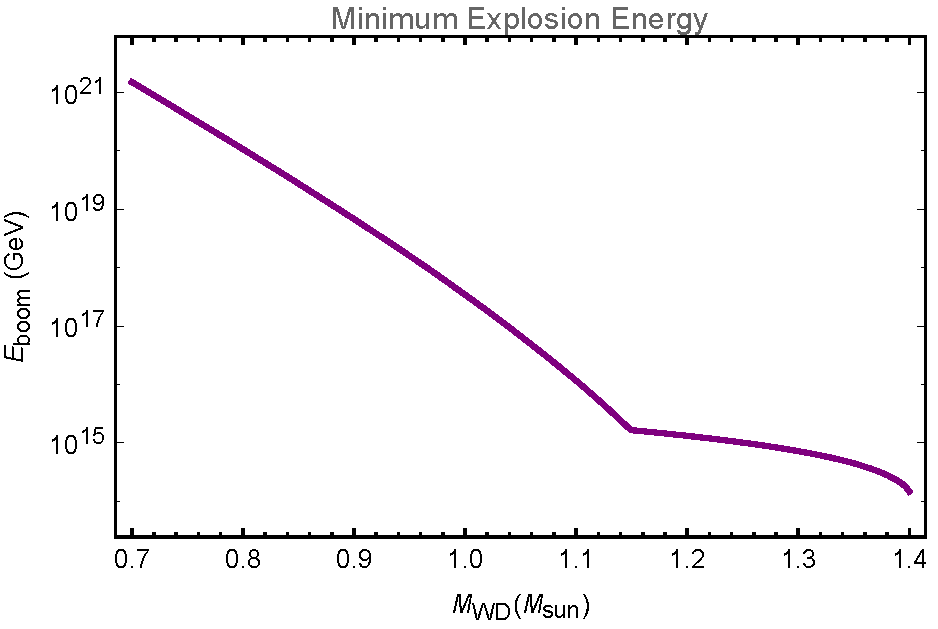
\includegraphics[scale=.45]{Eboom.pdf}
\caption{Minimum energy required to trigger explosion in a WD, based on numerical results for $\lambda_T$ \cite{Woosley}.}
\label{fig:Eboom}
\end{figure}

\section{Dark Matter Explosiveness}
\label{sec:DMexplode}
In this section, we parameterize the explosive power of a generic (ultra-heavy) DM interaction in the WD which releases $n_i$ SM particles of species $i$ each with kinetic energy $\epsilon$. 
\subsection{DM Transit}
Consider a DM transit through the WD, interacting with stellar constituents in a general manner as shown in Figure \ref{fig:feynmandiag}. The cross section for this interaction is denoted as $\sigma_{i,\epsilon}$. 
\begin{figure}
\label{fig:feynmandiag}
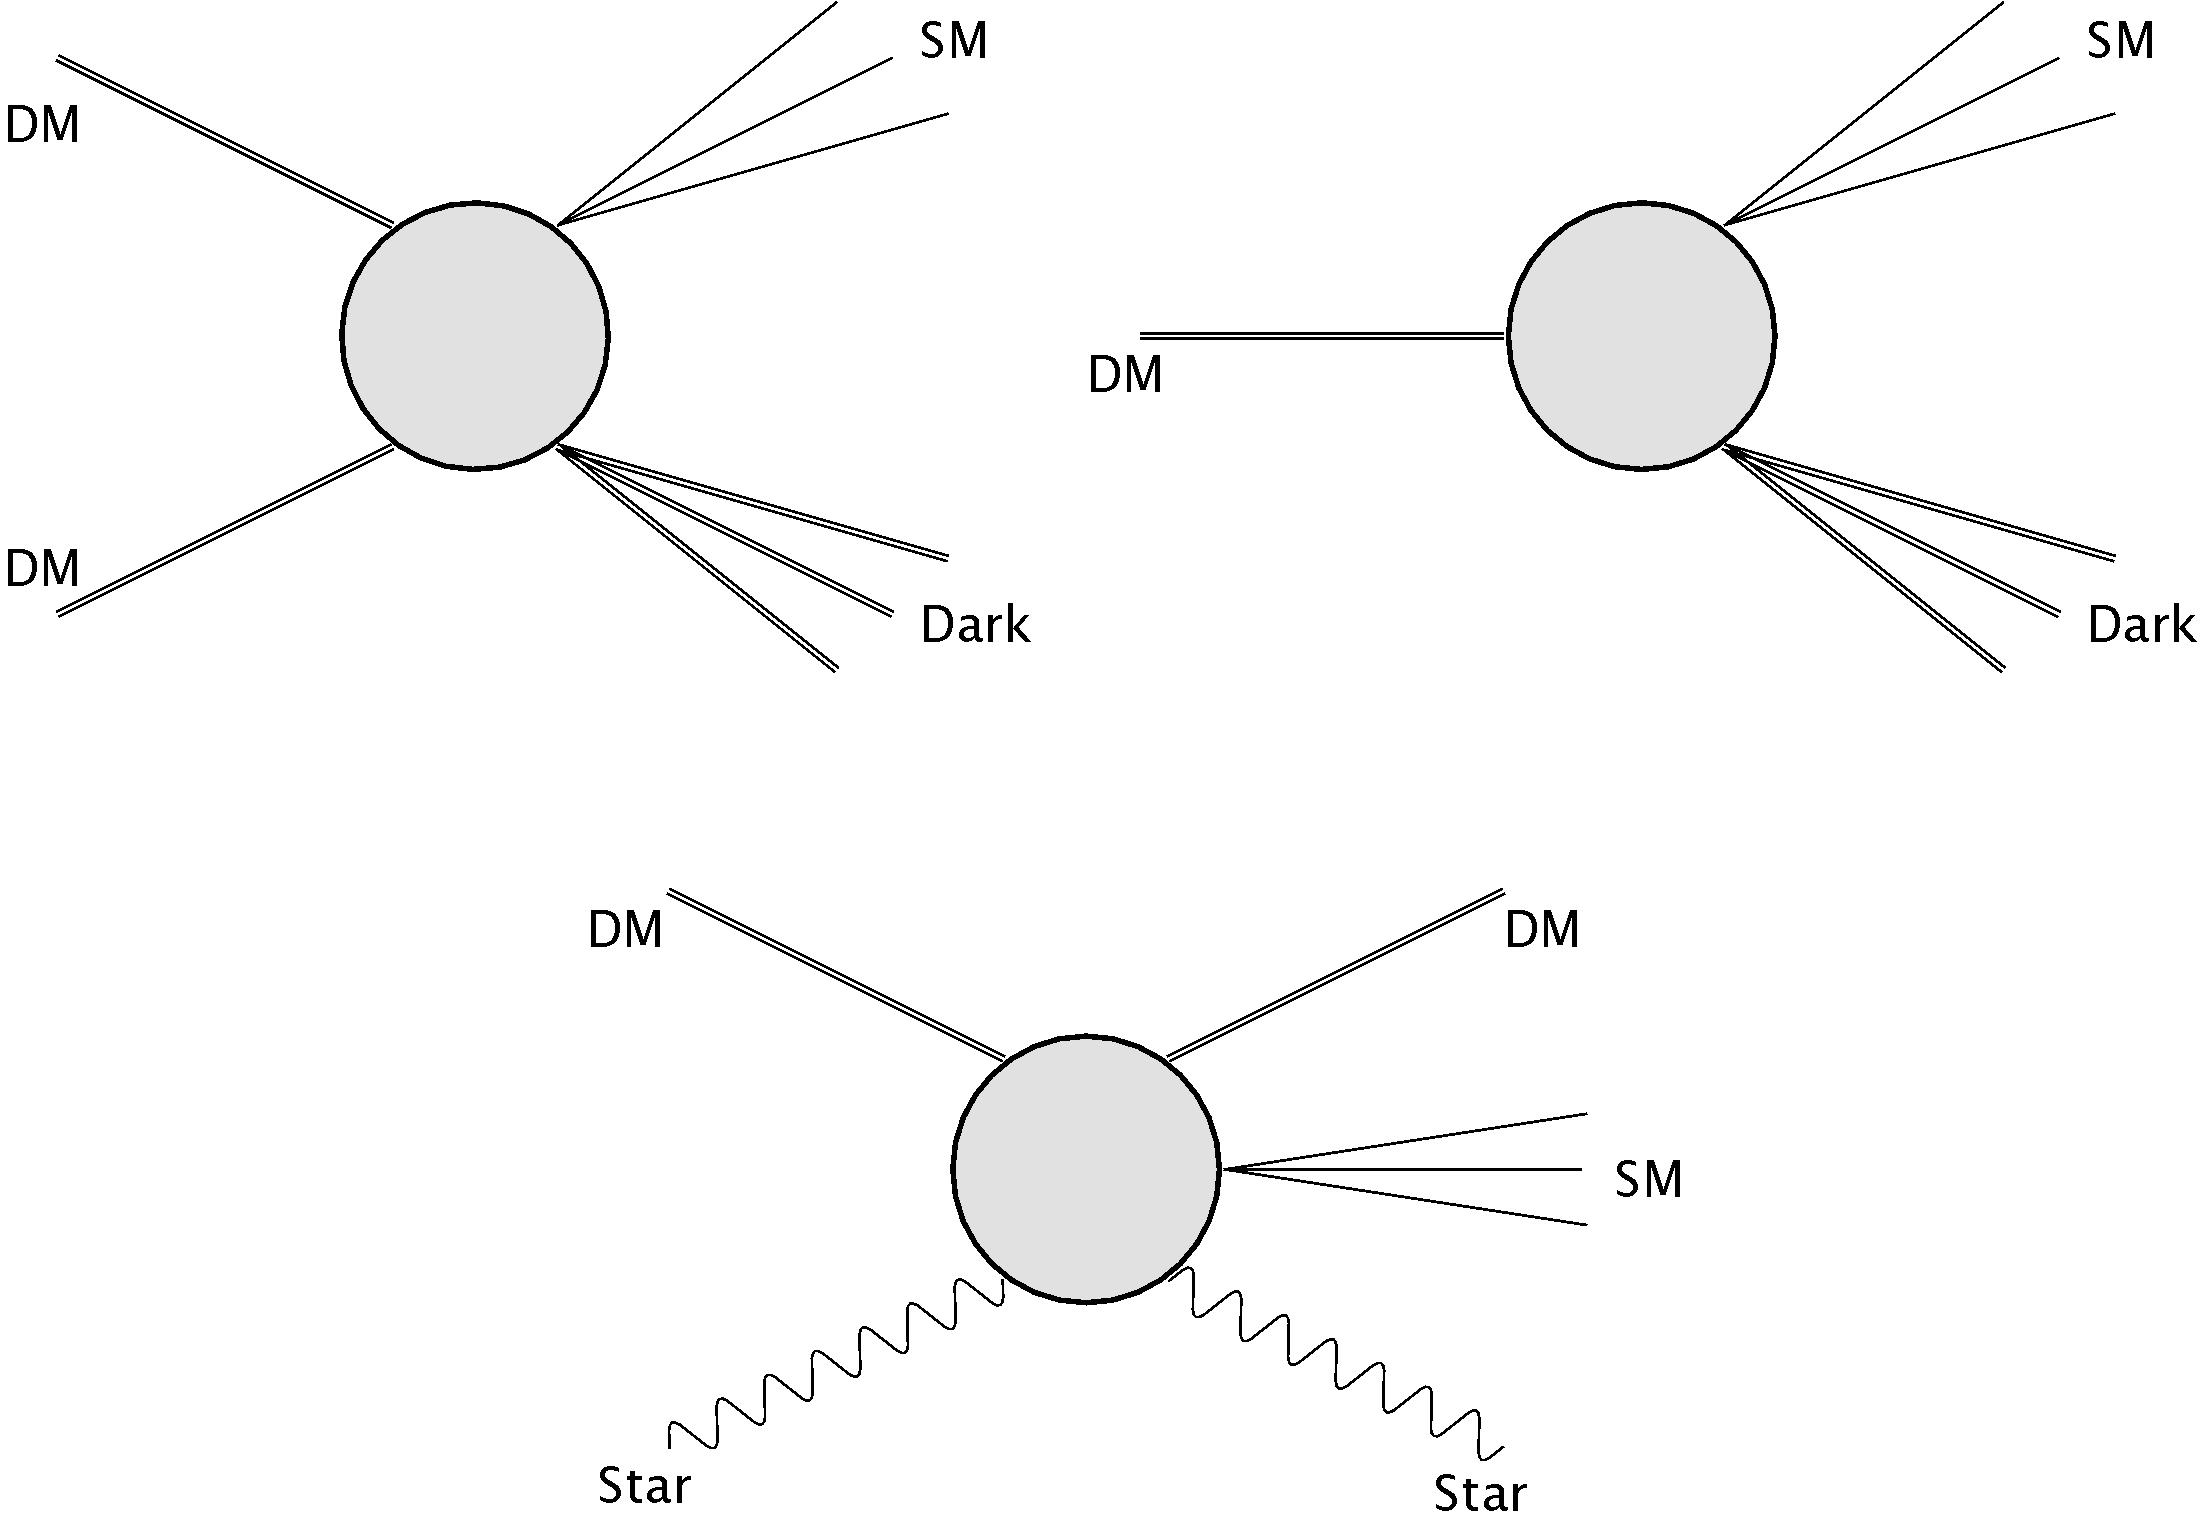
\includegraphics[scale=.05]{feynmandiag}
\caption{General interaction between ultra-heavy DM and WD constituents, producing $n_i$ additional particles of species $i$.}
\end{figure} 
Setting the total energy released during a transit of length $\text{max}\{\lambda_T, L\}$ to be greater than the explosive energy \eqref{eqn:boom}, we find a lower bound on the interaction cross section sufficient to trigger runaway fusion:
\begin{equation}
\label{eq:transitexplosion}
n_i \sigma_{\epsilon,i} \gtrsim \left\{
        \begin{array}{ll}
            \displaystyle \lambda_T^2 \l \frac{T_f}{\epsilon} \r & \quad L < \lambda_T \\
             \lambda_T^2 \l \frac{L}{\lambda_T}\r^2 \l \frac{T_f}{\epsilon} \r & \quad L > \lambda_T
        \end{array}
    \right..
\end{equation}

Note that in deriving \eqref{eq:transitexplosion}, we require that the DM transit time is less than the diffusion time corresponding to the explosive temperature profile. This results in the condition
\begin{equation}
\tau_d \gtrsim \frac{\text{max}\{\lambda_T, L\}}{v_\text{esc}},
\end{equation}
where $\tau_d$ is the characteristic time for a region of size $\text{max}\{\lambda_T, L\}$ and temperature $T_f$ to diffuse $\OO(1)$ of its heat, and $v_\text{esc}$ is the DM transit velocity (set by the escape velocity of the WD). An estimate from the heat equation yields $\tau_d \sim \frac{\lambda_T^2}{\alpha}$, where $\alpha$ is the (temperature-dependent) diffusivity. \textcolor{red}{Show condition is true for all densities.} Similarly, we also require that the time to transfer energy $\epsilon$ out to the initial temperature profile of length $L$ is less than the diffusion time scale $\tau_d$. Both of these conditions are necessary to ensure that energy depositions from individual collisions add coherently into a temperature profile during the full transit length. While a heating event can still be explosive if either of these conditions are violated, the formalism of \eqref{eq:transitexplosion} no longer holds in this case. 

In addition, we require that a DM with this interaction makes it through the crust of the WD of size of density $n_{\text{c}}$ and size $R_{\text{c}}$:
\begin{equation}
n_i \sigma_{\epsilon,i} \lesssim \l \frac{m_{\text{DM}} v_{\text{esc}}^2}{n_{\text{c}} R_{\text{c}}} \r \frac{1}{\epsilon}.
\end{equation}
Imposing \eqref{eq:transitexplosion}, we find lower bound on $m_{\text{DM}}$ such that the DM is able to both penetrate the crust \emph{and} trigger an explosion:
\begin{equation}
\label{eq:transitmass}
m_{\text{DM}} \gtrsim  T_f ~\text{max}\{\lambda_T, L\}^2 \l \frac{n_{\text{c}} R_{\text{c}}}{v_{\text{esc}}^2} \r
\end{equation}
If \eqref{eq:transitmass} is violated, than the DM interaction is either not strong enough to ignite the WD or it is too strong that it has no chance to transit the interior as it gets stopped in the crust. In the case of $\lambda_T > L$, this translates to a model-independent lower-bound on the DM mass $\sim 10^{27} - 10^{34} ~\GeV$. \textcolor{blue}{used 1 km crust and same number density as interior}. 

We now calculate the maximum possible DM mass that may transit a single WD within its lifetime $\sim \text{Gyr}$. The expected transit rate for an ultra-heavy DM state is given by
\begin{equation}
\Gamma_\text{DM} = n_\text{DM} \sigma_g v \sim \frac{\rho_{\text{DM}}}{m_\text{DM}} \pi R_{s}^2 \l\frac{v_\text{esc}}{v}\r^2 v,
\end{equation}
where $v \sim 10^{-3}$ is the virial velocity of DM and $\rho_{\text{DM}}$ is the energy density of DM in the region of interest. $\sigma_g$ denotes the capture cross section including a gravitational Sommerfeld enhancement. Considering a $1.25 M_{\odot}$ WD in the local dark matter halo $\rho_{\text{DM}} \sim 0.3 ~\text{GeV}/\text{cm}^3$, we find that $m_\text{DM} \lesssim 10^{44} ~\GeV \sim 10^{20} ~\text{g}$ will transit the WD at least once in a Gyr. If we instead consider (recently discovered) heavy white dwarfs in the galactic center $\rho_{\text{DM}} \sim 10^3 ~\text{GeV}/\text{cm}^3$, this upper bound improves to $m_\text{DM} \lesssim 10^{48} ~\GeV \sim 10^{24} ~\text{g}$. 
\textcolor{blue}{Hard to put this into ``scaling" notation}. 

\subsection{DM-DM Collisions}

\section{Heating Length}
\label{sec:heatinglength}
For the DM interactions under consideration, the released energy must be efficiently transferred to the WD in order to trigger runaway fusion. We define $R_{i, \epsilon}$ as the distance over which a particle species $i$ and any secondaries transfer $\OO(1)$ of the initial energy $\epsilon$ to stellar constituents. In this section, we summarize the available modes of energy loss for different SM particles in a WD and compute the deposition length $R_{i, \epsilon}$ in each case. Detailed calculations of the various interactions are presented in Section \ref{sec:appendix}. For a given process, $R_{i, \epsilon}$ will be directly related to the heating length $L$ in a straightforward manner. As we are primarily concerned with depositing sufficient energy to ignite supernovae, we focus on high-energy particles $\epsilon \gg T_f$ which interact via the strong and electromagnetic forces (i.e. electrons, muons, photons, pions, and neutral hadrons). In this way, the WD may be thought of as a ``particle detector" with electromagnetic and hadronic ``calorimeter" components. 

\subsection{Electrons and Photons}

\subsection{Heavy Charged Particles}

\subsection{Hadrons}

\begin{figure}
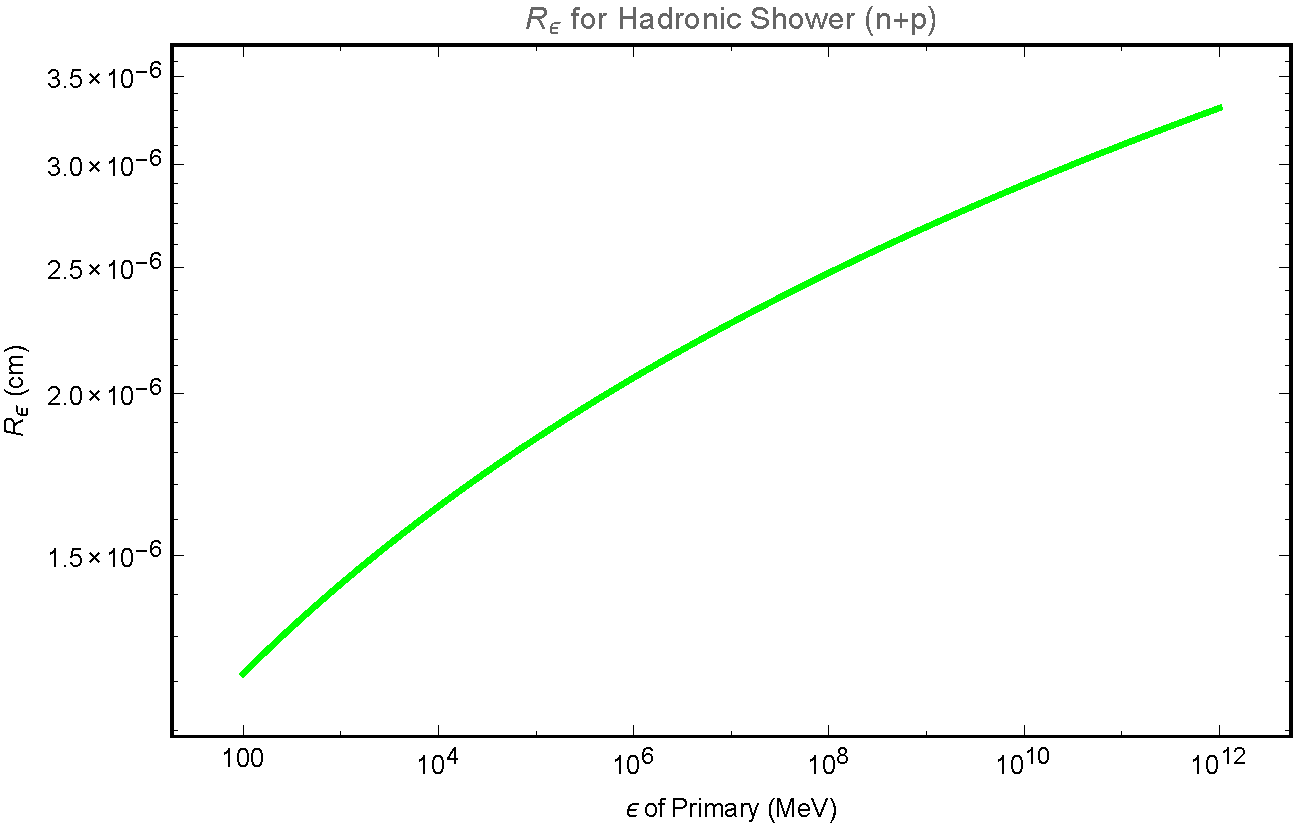
\includegraphics[scale=.35]{hadronic.pdf}
\end{figure}

\section{Q-balls}
\label{sec:Qballs}
In various supersymmetric extensions of the standard model (SM), non-topological solitons called Q-balls can be produced in the early universe \cite{Coleman:1985ki, Kusenko:1997si}. If these Q-balls were stable, they would comprise a component of the dark matter today. In gauge-mediated models with flat scalar potentials, the Q-ball mass and radius are given by
\begin{equation}
\label{eq:Qballprop}
M_Q \sim m_F Q^{3/4}, ~~~ R_Q \sim m_F^{-1} Q^{1/4},
\end{equation}
where $m_F$ is related to the scale of supersymmetry breaking (messenger scale). The condition $M_Q/Q < m_p$ ensures that the Q-ball is stable against decay to nucleons \cite{Dine:2003ax}. When an (electrically neutral) baryonic Q-ball interacts with a nucleon, it absorbs its baryonic charge as a minimum-energy configuration and induces the dissociation of the nucleon into free quarks. During this process, $\sim \text{GeV}$ of energy is released through the emission of 2-3 pions \cite{Dine:2003ax}. The cross section for this interaction is approximately geometric:
\begin{equation}
\sigma_Q \simeq \pi R_Q^2.
\end{equation}
Note that a sufficiently massive Q-ball will become a black hole if the Q-ball radius is less than the Schwarzschild radius $R_Q \lesssim R_s \sim G M_Q$. In the model described above, this translates into a condition
\begin{equation}
m_F \l\frac{\Mpl}{m_F}\r^3 \lesssim m_Q, ~~~ \l\frac{\Mpl}{m_F}\r^4 \lesssim Q.
\end{equation}
For Q-ball masses of this order, gravitational interactions become relevant. 

We assume that for each Q-ball collision, there is equal probability to produce $\pi^0, \pi^+$ and $\pi^-$ under the constraint of charge conservation. In the notation of Section \ref{sec:DMexplode}, this results in $n_{\pi} \sim 10$ pions released with $\epsilon \sim 500 ~\text{MeV}$. The mean distance travelled by a relativistic particle before decaying is $d = \gamma v \tau$. For neutral pions $d_{\pi^0} \sim 10^{-5} ~\text{cm}$ while for charged pions, $d_{\pi^\pm} \sim 10 ~\text{m}$. Numerous experiments have studied the effects of $50 - 500 ~\text{MeV}$ pions incident upon complex nuclei targets such as carbon. It is found that there is roughly equal cross section of order $\OO (100 ~\text{mb})$ for a (neutral or charged) pion to either scatter elastically, scatter inelastically, or become absorbed with no final state pion \cite{Pionnuclear}. Of these possibilities, pion absorption is the most relevant for energy loss as this will induce a hadronic shower.

Q-balls that transit a WD with sufficiently large cross section as given by \eqref{eq:transitexplosion} will ignite the star. Following the results of Section \ref{sec:heatinglength}, we find that the relevant heating length $L$ of the Q-ball interaction is simply. The resulting explosive power for Q-balls is plotted in Figure \ref{fig:boomQball}. If the Q-ball cross section is related to its mass and baryonic charge as in \eqref{eq:Qballprop}, we find that
\begin{equation}
m_Q \gtrsim 10^8 ~\text{g} \l\frac{m_F}{\text{TeV}}\r^4, ~~~~ Q \gtrsim 10^{38} \l\frac{m_F}{\text{TeV}}\r^4
\end{equation}
is capable of triggering runaway fusion in a heavy $\sim 1.25 M_{\odot}$ WD. 

\begin{figure}
\label{fig:boomQball}
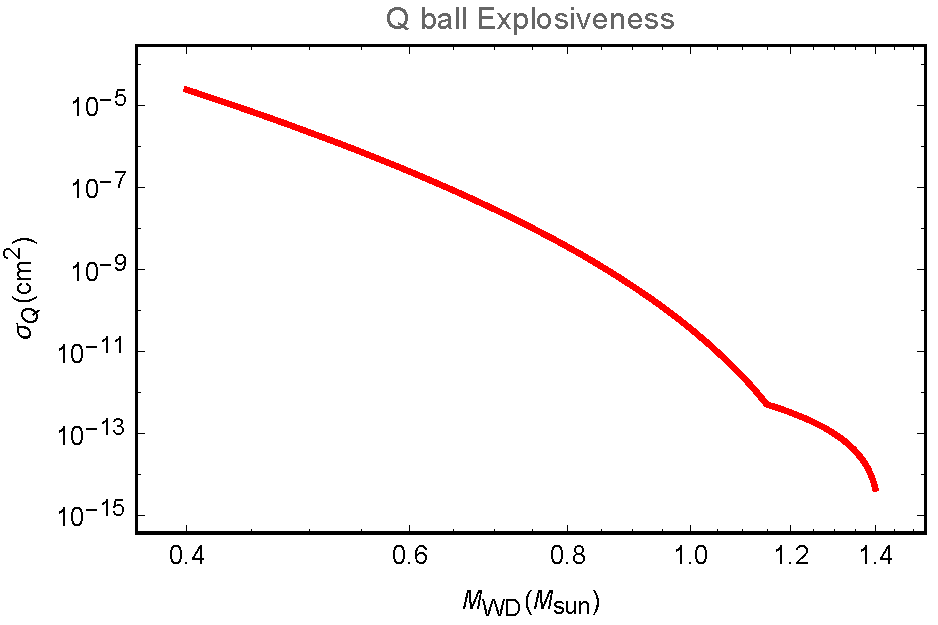
\includegraphics[scale=.45]{boomQball.pdf}
\end{figure}

\textcolor{blue}{Need to implement SN rate and transit rate here...} \textcolor{blue}{Triangle Plot of Q-ball constraints vs. terrestrial}. 

\section{Discussion}
\label{sec:discussion}

\begin{appendices}

\section{Particle Interactions in a White Dwarf}
\label{sec:appendix}

The interior of a WD is a complex environment (unless otherwise noted, we will assume a carbon-oxygen WD). Famously, the star is supported against collapse by electron degeneracy pressure with a characteristic Fermi energy $E_F \sim n_e^{1/3}$, where $n_e$ is the number density of electrons. In addition, the nuclei are at an ambient temperature $T \sim \text{keV}$ and form a strongly-coupled plasma with plasma parameter
\begin{equation}
\frac{Z e^2}{n^{1/3} T} \gg 1,
\end{equation}
where $n$ is the number density of nuclei. Here we provide a detailed analysis of the possible electromagnetic and strong interactions in a WD. 

\subsection*{Coulomb Collisions}

Generically, an incident (spin-0) particle of mass $m_i$, charge $e$, and velocity $\beta$ scattering off a (stationary) target of mass $m_t$, charge $Ze$ is described by the differential cross section
\begin{equation}
\label{eq:rutherford}
\frac{d \sigma}{dE'} = \frac{2 \pi  \alpha^2 Z^2}{m_t \beta^2} \frac{1}{E'^2} \l1- \frac{\beta^2 E'}{E_{\text{kin}}}\r,
 \end{equation}
where we have assumed a sufficiently fast incident particle so that interactions are governed by single collisions with energy transfer $E'$ \cite{Agashe:2014kda}. $E_{\text{kin}}$ denotes the maximum energy transfer possible satisfying kinematic constraints:
\begin{equation}
E_{\text{kin}} = \frac{2 m_t \beta^2 \gamma^2}{1+ 2\gamma(m_t/m_i) +(m_t/m_i)^2},
\end{equation}
where $\gamma = (1-\beta^2)^{-1/2}$ is the relativistic factor.

For sufficiently heavy incident particles, the differential cross section depends only on the velocity of the incident particle. Note that higher-spin particles receive additional corrections to the cross section, but for small energy transfers these corrections are negligible. It is straightforward to understand the parametric dependences of \eqref{eq:rutherford}: there is increased likelihood to scatter for slowly moving incident particles undergoing ``soft-scatters" against lighter targets. Therefore, one would expect that soft scattering dominates the energy loss and that collisions with nuclei of mass $M$ are suppressed by a factor $\OO\l\frac{Z m_e}{M}\r$ as compared to collisions with electrons. This is certainly true for incident charged particles in non-degenerate matter. However, both of these naive expectations turn out to be false when considering scattering off a degenerate species.

We first consider the energy loss from scattering high-energy charged particles off non-degenerate targets. In this case, the stopping power due to collisions with a number density $n$ is given by:
\begin{align}
\label{eq:SP}
\frac{dE}{dx} & = - \int dE' \left(\frac{d \sigma}{dE'}\right) n E' \\
& \sim -\frac{n Z^2 \alpha^2}{m_t \beta^2} \log{\l\frac{E_{\text{max}}}{E_{\text{min}}}\r}.
\end{align}
\eqref{eq:SP} must be integrated over all $E'$ within the regime of validity for \eqref{eq:rutherford}, thereby fixing the lower and upper bounds of the Coulomb logarithm. Quantum mechanical uncertainty sets a limit to the accuracy that can be achieved in ``aiming" an incident particle at a target. In terms of the collisional impact parameter $b$, this results in a bound $b > \frac{1}{\text{min}\{{m_i, m_t}\} \beta \gamma}$ and in terms of energy transfer, this translates to the condition
\begin{equation}
E' < E_q \sim \frac{Z^2 \alpha^2 \gamma^2 ~\text{min}\{{m_i, m_t}\}^2}{m_t}.
\end{equation}
In addition, the expression for the differential cross section \eqref{eq:rutherford} no longer holds when $E'$ becomes larger than the mass of the target \cite{Rossi}. For our calculations, we take the maximum energy that an incident particle is able to transfer to be
\begin{equation}
E_{\text{max}} = \text{min}\{E_q, E_{\text{kin}}, m_t\}.
\end{equation}
On the other hand, the maximum impact parameter is set by Thomas-Fermi screening due to the degenerate electron gas:
\begin{equation}
\lambda_{\text{TF}} \sim \l \frac{Z e^2 n_e}{E_F}\r^{-1/2},
\end{equation}
This corresponds to a lower bound
\begin{equation}
E_{\text{sc}} \sim \frac{m_e^2 Z^2 \alpha^2}{m_t \beta^2}.
\end{equation}
However, the lattice structure of ions in the WD introduces further complications \cite{Teukolsky}. The typical Coulomb lattice binding energy between ions of number density $n$ is given by the electric potential
\begin{equation}
\label{eq:lattice}
E_B \sim \frac{Z^2 e^2}{n^{-1/3}}.
\end{equation}
For energy transfers greater than $E_B$, any lattice effects can be safely ignored. On the other hand, momentum transfers from collisions below this threshold will lead to suppressed energy loss due to collective effects. For simplicity we set the lower bound on nuclei scattering (not applicable for electron targets) to be
\begin{equation}
E_{\text{min}} = \text{max} \{E_B,E_{\text{sc}}\}
\end{equation}
so that we only account for energy transfers greater than the ionic lattice binding energy.

Now consider collisions with degenerate electrons. An incident particle transferring energy $E'$ can only scatter those electrons within $E'$ of the Fermi surface. We define a modified density of electrons $n_e(E')$ as:
\begin{equation}
n_e(E') = \left\{
        \begin{array}{ll}
            \displaystyle \int \limits_{E_F -E'}^{E_F}dE ~g(E) & \quad E' \leq E_F \\
            n_e & \quad E_F \leq E'
        \end{array}
    \right.,
\end{equation}
where $g(E)$ is the density of states per unit volume for a three-dimensional free electron gas. The effect of degeneracy can also be cast as a suppression of the differential cross section of order $\mathcal{O}(E'/E_F)$ whenever energy less than $E_F$ is transferred. Therefore, unlike in the non-degenerate case, the energy loss due to soft-scatters are in fact \emph{subdominant} to the contributions from rare hard-scatters. The stopping power is also sensitive to the integration bounds $E_{\text{max}}$ and $E_{\text{min}}$ as a power-law dependence unlike the logarithmic sensitivity \eqref{eq:SP} in the case of a non-degenerate target. 

\subsection*{Bremsstrahlung and Pair Production}

\subsection*{Nuclear Interactions} 

Nuclear interactions in the WD can be either elastic or nonelastic scatters. Each elastic scatter transfers a fraction $\sim \l1-\l\frac{m}{m + M}\r^2\r$ of the incident energy (averaging over scattering angles), where $m$ and $M$ are the masses of the incident hadron and nuclei respectively. However, the ``Coulomb lattice" of ions in the WD (see \eqref{eq:lattice}) implies that elastic collisions do not transfer energy less than $E_B$. This sets a lower bound on the energy loss function for elastic scatters, which is of the form

The cross section for elastic scatters has considerable dependence on the hadron species. For neutrons and protons, the nuclear elastic cross section is of order $\sigma_\text{el} \sim 100 ~\text{mb}$ for energies greater than $\text{MeV}$. However at lower energies, the elastic cross section effectively vanishes for protons but rises to $\OO(\text{b})$ for neutrons. This can be understood physically as charged hadrons may only elastically scatter off nuclei if the incident energy is sufficient to overcome the mutual Coulomb barrier. Also note that for incident energies below an $\text{MeV}$, the neutron capture cross section is negligible compared to the elastic cross section. We find that $\OO(10)$ elastic scatters are needed to ``moderate" neutrons from 5 MeV to 1 MeV in the WD. This final-step will necessarily take the form of a random-walk.

For the purpose of energy deposition, elastic scatters are far subdominant to nonelastic scatters. For a particle $i$ of incident energy greater than the nuclear binding energy $E_\text{nuc} \sim 10 ~\text{MeV}$, nonelastic nuclear interactions typically result in an $\OO(1)$ number of energetic secondary hadrons (i.e. protons, neutrons, pions, etc.) emitted roughly in the direction of the primary particle. These secondary particles approximately split the initial total energy of the absorbed primary particle and can collide with other nuclei in the WD. In addition, the nucleus will generally be left in an excited state and relax through the emission of low-energy $\OO(10 ~\text{MeV})$ nucleons (``nuclear evaporation") and photons \cite{Rossi}. The cross section for any such process is approximately set by the nuclear length scale $\sim \text{fm}$. A hadronic shower is a result of all such reactions caused by primary and secondary particles.

To estimate the typical shower length $X_{\text{had}}$, we assume a model in which a primary particle of energy $\epsilon$ interacting with nuclei to produces $N$ secondary particles each of energy $\epsilon/N$ (we ignore the effects of the evaporative stage in each reaction as this will only introduce minor corrections at sufficiently large $\epsilon$). The shower will end once final-state hadrons reach a critical energy $E_c$ - this is either set by the scale at which an additional mechanism dominates the stopping power or the minimum energy required to induce further showers $E_\text{nuc}$. According to this model, we find a hadronic shower length 
\begin{equation}
X_{\text{had}} = l_i + l_\text{had} \l \frac{\log{(\epsilon/E_c)}}{\log{N}}\r,
\end{equation}
where $l_i$ is the nuclear mean free path for incident particle $i$. Note that the shower length has a mild, logarithmic sensitivity to the initial energy $\epsilon \gg ~\text{10 ~\text{MeV}}$ and number of secondaries and is therefore primarily set by the nuclear mean free paths. In the case of an incident hadron (proton, neutron, pion), the hadronic shower length is approximately set by a single length scale $X_{\text{had}} \approx 10 ~l_\text{had}$. 

There is considerable uncertainty in the evaluation of nuclear mean free paths for high-energy particles. In fact, the cross sections under considerations generally rise with increasing energy, although this precise relation is beyond the scope of this work. Instead, we will approximate the relevant nuclear cross sections to be constant. As a conservative estimate, we take the nonelastic cross sections for hadrons and photons interacting with nuclei to be 
\begin{equation}
\sigma_{had-A} \sim 100 ~\text{mb}, ~~~\sigma_{\gamma-A} \sim 1 ~\text{mb}.
\end{equation}

Charged leptons can also lose energy via electronuclear interactions in which an incident electron or muon radiates a virtual photon that then interacts hadronically with a nearby nucleus. In this case, it is more appropriate to describe the interaction as a radiative stopping power. This has been computed in \cite{Gerhardt:2010bj} in terms of the photonuclear mean free path:
\begin{equation}
\l \frac{dE}{dx}\r_{e-A} \sim E \l \frac{\alpha}{l_\gamma}\r
\end{equation}

The end products of a hadronic shower will generally be hadrons of kinetic energy $1-10 ~\text{MeV}$ which are incapable of inducing further nuclear disintegration. Charged hadrons have appreciable electromagnetic interactions with nuclei, while collisions with degenerate electrons are completely screened at these energies. We find that $\OO(10)$ elastic scatters are needed to ``moderate" neutrons from 5 MeV to 1 MeV in the WD. This final-step will necessarily take the form of a random-walk. Charged hadrons have appreciable electromagnetic interactions with nuclei, while collisions with degenerate electrons are completely screened at these energies. On the other hand, electromagnetic couplings are highly suppressed for final-state neutral hadrons. The dominant source of energy loss for neutrons in this range is elastic scattering off nuclei 


\end{appendices}

\section*{Acknowledgements}
We are grateful to S. Rajendran for suggestions and collaboration during the early stages of this work, as well as his ``benign negligence". We would also like to thank D. Grabowska, K. Harigaya, R. McGehee, and J. Wurtele for stimulating discussions.

\bibliography{Qballs}

\end{document}
